\subsection{Termometro elettronico}


\begin{figure}[ht]
 \centering
   {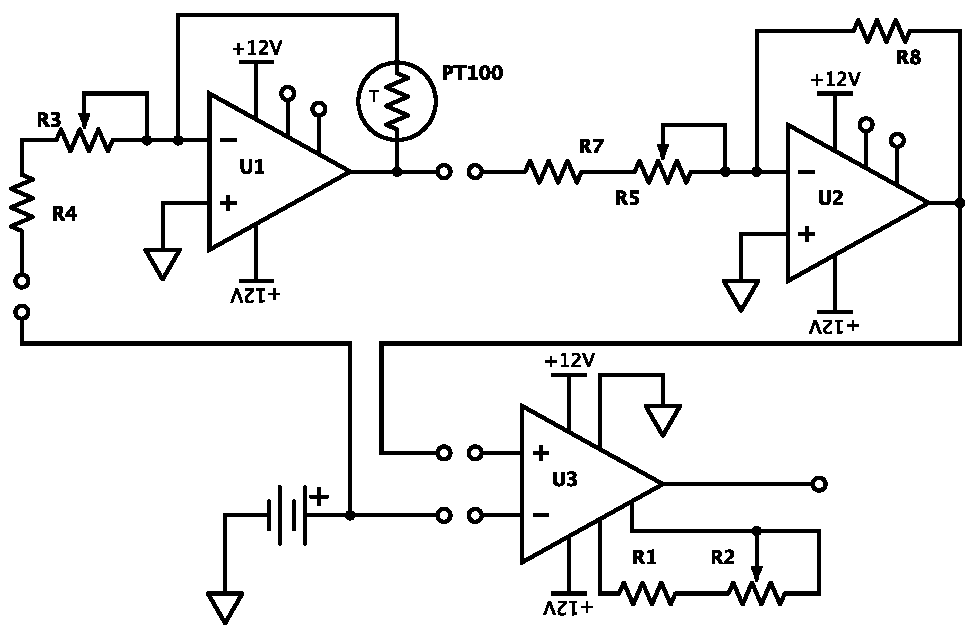
\includegraphics[width=0.75\textwidth]{../E06/latex/c1.pdf}}
 \caption{Schema circuitale del termometro elettronico.}
 \label{gr5:sbil_amp_diff}
\end{figure}


In questa prima parte vogliamo realizzare un termometro elettronico. Per far ciò usiamo una termoresistenza Pt100 di resistenza 100\si{\ohm} a zero gradi Celsius. Il nostro circuito sarà realizzato a blocchi, metodo migliore per realizzare circuiti complessi.
\subsubsection*{Conversione Resistenza-Tensione}
Per convertire la variazione di resistenza della nostra Pt100 in tensione dobbiamo far scorrere in essa una corrente, scelta di \SI{1}{\milli\ampere} per evitare autosurriscaldamenti. 

\subsubsection*{Amplificazione e Condizionamento del segnale}
Vogliamo poi ottenere una lettura di tensione pari a 0 quando la temperatura ambientale è di $0^{\circ}C$ e una $\Delta V=100\si{\milli\volt}/^{\circ}C$.




\subsubsection{Generatore di corrente costante [Blocco 1]}

\begin{wrapfigure}[13]{r}{0.45\textwidth}
\centering
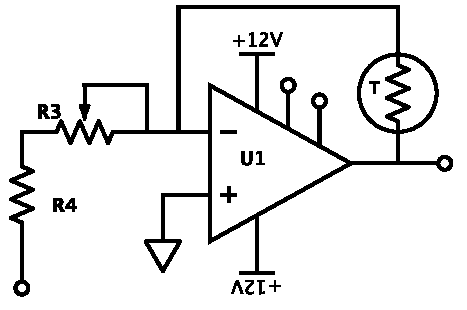
\includegraphics[width=.25\textwidth]{../E06/latex/P1.pdf}
\caption{Blocco 1: Generatore di corrente costante.}
\label{cir5:2wire}
\end{wrapfigure}


Come primo blocco realizziamo un generatore di corrente costante. Come sappiamo, la tensione che scorre nel ramo di retroazione è univocamente determinata dalla tensione all'ingresso invertente e dalla resistenza $R_4+R_3$ (Dobbiamo solo stare attenti che il nostro opamp non vada in saturazione. In questo caso la corrente dipenderà dal carico). Infatti, da una semplice analisi circuitale, otteniamo che $I=V_{in}/(R_4+R_3)$. È stato scelto di utilizzare come resistenza all'ingresso invertente un resistenza da $4.7\si{\kilo\ohm}$ con in serie un trimmer multigiro da $1\si{\kilo\ohm}$. Così facendo, utilizzando un amperometro in serie, possiamo tarare con precisione la corrente che scorre nel ramo di retroazione (e dunque nella nostra termoresistenza). Durante questa fase non utilizzeremo la termoresistenza (perchè in caso di errori nel circuito potremmo rovinarla ed è alquanto costosa) ma una resistenza di $100\si{\ohm}$. Come già detto la corrente scelta è stata di \SI{1}{\milli\ampere}. Con tale scelta la potenza dissipata dalla nostra termoresistenza è $P=\frac{I^2}{R}$. Inserendo i valori numerici otteniamo $P=0.1\si{\milli\watt}$.  

Per la tensione $V_{in}$ utilizzeremo un generatore di tensione di riferimento +5\si{\volt} REF02, che garantisce una tensione costante con un incertezza di $0.3\%$.

\subsubsection{Amplificazione [Blocco 2]}

\begin{wrapfigure}[13]{r}{0.45\textwidth}
\centering
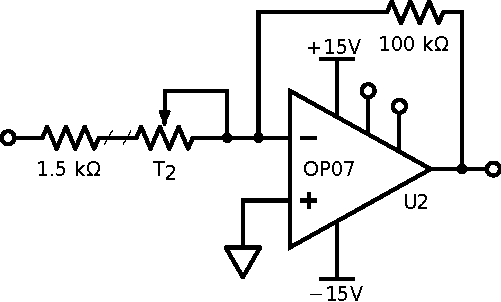
\includegraphics[width=.25\textwidth]{../E06/latex/P2.pdf}
\caption{Blocco 2: Amplificatore con G=50.}
\label{cir5:2wire}
\end{wrapfigure}


La tensione in uscita dal blocco 1 è $100 \si{\milli\volt}$ a $0^{\circ}C$ e una variazione per ogni grado centigrado di $\Delta V=0.385\si{\milli\volt}/^{\circ}C$. Ciò che vogliamo ottenere è una tensione di $0 \si{\milli\volt}$ a $0^{\circ}C$ e un $\Delta V=100\si{\milli\volt}/^{\circ}C$, così da avere una conversione in gradi centigradi a meno di un fattore 10. Desideriamo dunque un'amplificazione di $G=\frac{100\si{\milli\volt}/^{\circ}C}{0.385\si{\milli\volt}/^{\circ}C}=259.740$. 


Come prima cosa amplifichiamo il segnale in uscita dal blocco 1. Vogliamo che quando siamo a $0^{\circ}C$ la tensione sia $5\si{\volt}$ blocco 2. Così facendo, possiamo usare un comparatore con $V_{ref}=5\si{\volt}$ che, trivialmente, restituirà in uscita $0\si{\volt}$ quando la temperatura è di zero gradi. 

Per tarare il Gain del nostro amplificatore (che ovviamente dovrà essere G=50), abbiamo deciso di utilizzare un segnale DC di $-100\si{\milli\volt}$ dall'Agilent portato all'ingresso invertente (l'ingresso non invertente è stato collegato a comune). Abbiamo utilizzato una resistenza di feedback di $100\si{\kilo\ohm}$ mentre la resistenza all'ingresso invertente è stata costruita mettendo in serie una da $1.5\si{\kilo\ohm}$ e un trimmer multigiro da $1\si{\kilo\ohm}$. Così facendo è stato possibile tarare perfettamente il guadagno a 50, che evidentemente si ha quando la tensione in uscita è $5\si{\volt}$. 

\subsubsection{Condizionamento [Blocco 3]}

\begin{wrapfigure}[13]{r}{0.45\textwidth}
\centering
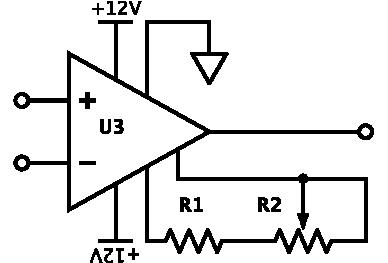
\includegraphics[width=.25\textwidth]{../E06/latex/P3.pdf}
\caption{Blocco 3: Amplificatore differenziale con G=5.195.}
\label{cir5:2wire}
\end{wrapfigure}


Portiamo ora tale segnale amplificato all'ingresso non invertente di un amplificatore per strumentazione (AD622) e utilizziamo come riferimento i $5\si{\volt}$ forniti dal generatore di tensione REF02. Quando l'ambiente si trova alla temperatura di $0^{\circ}C$, la tensione in uscita dal blocco 2 è proprio $5\si{\volt}$ e dunque l'AD622 avrà un' uscita nulla. Quando la temperatura è maggiore di zero anche l'uscita del blocco 3 sarà maggiore di zero, perchè la tensione all'ingresso non invertente (segnale della temperatura) è maggiore del riferimento ($5\si{\volt}$). Dobbiamo ora decidere a quanto settare il guadagno del nostro AD622. Per far ciò basta ricordare che il guadagno totale, ovvero il prodotto del guadagno di U2 e di U3 deve valere $G=259.740$. È dunque immediato verificare che $G_{U3}=5.195$. Utilizzando la formula $G=1+\frac{50.5k\Omega}{R_g}$ possiamo ottenere il valore di resistenza di gain: $R_g=12.038\si{\kilo\ohm}$. Utilizzando dunque la serie tra una resistenza da $10\si{\kilo\ohm}$ e un trimmer multigiro da $10\si{\kilo\ohm}$, con l'ausilio del multimetro digitale, abbiamo tarato tale resistenza. 

Per essere sicuri che il guadagno fosse esattamente quello cercato, abbiamo fornito all'ingresso non invertente una tensione di $6\si{\volt}$ e controllato che l'uscita fosse $V_{out}=5.195 \si{\volt}$. 

Controllati dunque tutti i moduli separatamente, abbiamo sostituito la resistenza da $100\si{\ohm}$ con la termoresistenza Pt100. La misura di tensione all'uscita è stata $V_{out}=(2.437\pm 0.002)\si{\volt}$. Come già detto, per ottenere la temperatura in gradi Celsius basta moltiplicare il valore di tensione per 10. La temperatura ambiente misurata risulta dunque $T=(24.37\pm0.02)^{\circ}C$.











